\newpage\EDJ{Please delete this newpage command later}
We provide three examples here for illustration and evaluation of our Coq plugin. 

\subsection{Type Safety for STLC}\EDJ{We need a fuller view of the two examples. Especially show "accessing family components outside that family".}
\label{sec:coqexample-stlc}

  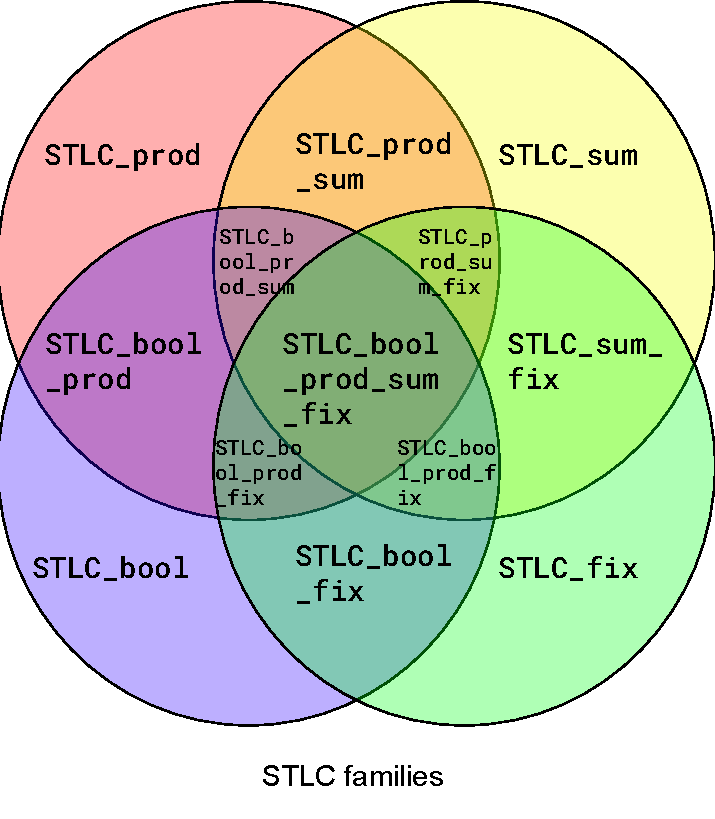
\includegraphics[width=0.5\textwidth]{coqexmaple/Mixin-Venn-Diagram.pdf}

The first example is the example throughout our paper---type safety proof of STLC, largely adapted
from Software Foundation~\cite{pierce2014software}. We singled out each language extensions from
STLC and prove the type safety for them separately, following
the style of the examples in MTC~\cite{delaware2013,forsta2020}.
And we use the \textbf{mixin} feature---that is capable of mixing two linkage transformer---to mix the semantics and properties of language features---product
, boolean (in \cref{fig:STLC-example}), sum type and iso-recursive type---with vanilla STLC.



% Using this example,
% we hope one day we can say precisely, \textit{a programming language feature itself is a
% piece of data/inheritance judgement/inherited family}. 
Compared with MTC,
our example uses small-step operational semantics\YZ{Does MTC not define a small-step operational semantics for STLC?}\EDJreply{I thought they use big step with fuel. Though Coq a la carte use small-step in one example} by exploiting
extensible inductive types. Most of the proof and computation are directly adapted from the one in Software Foundation, resulting in a similarly accessible proof. However, we highlight some special expriences when using our plugin. 

\begin{minted}[fontsize=\footnotesize]{Coq}
Lemma subst_on_true : forall G, hasty G (subst tm_true x k) ty_bool.
Overridable pins {step} FClaim not_step_tm_true: forall x', ~ step tm_true x' 
    by { intros x' h; inversion h }.
\end{minted}

Our proof is \textbf{more modular} as each part handling the extended feature are scattered in the extended families.


We use \textbf{propositional computational axiom} when computing "FRecursion". For example, when we prove or extend substitution lemma for bool, we need to prove a subgoal like "subst_on_true" requiring a computation based on the definition of "subst". In vanilla Coq, that can be easily done via "simpl" but in our case, we need to use the postulated computation axiom to simplify the computation of "subst" instead.

We handle \textbf{inversion lemma} differently. Inversion lemmas are those small lemmas while involving global reasoning. One example is "not_step_tm_true" which trivially asserts "tm_true" is not further reducible. It requires global reasoning because once the user errorneously add a constructor for "step tm_true tm_true" then this lemma cannot hold. Thus one way is to prove it by "FInduction" on the "step".  However, this brings a lot of boilerplate code as everytime "step" is extended with some unrelated constructor (e.g. "st_if : step (tm_if tm_true b c) b"), "not_step_tm_true" needs to be extended correspondingly---we need to check "st_if" doesn't "step tm_true" requiring using \textbf{partial recursor and the computational axiom} to prove "(tm_if tm_true b c) <> tm_true" syntactically speaking using tactic "fdiscriminate".

Thus we provide a small-scale \textbf{escape hatch via "Overridable"}. Once "pins {step}", we will know the \textit{concrete} (vanilla Coq) inductive type of "step" when proving "not_step_tm_true" and thus we can use all Coq's induction facility including "inversion". Once the definition of "step" extends during inheritance, due to the semantic of "Overridable", we need to provide a new proof but our plugin can also try to use the old proof script automatically. This trick can apply to small inversion lemma where we believe our inductive definition is ``well-formed'' enough and thus an "inversion" tactic can easily handle it. Another way to look at it is the fact that, this kind of inversion lemma should be part of the definition in the first hand, like a constraint---and the proof that our inductive definition satisfy this constraint should be trivial and any future extension should respect this constraint.

% One kind of examples is about the computation, for example, substitution functions. Substitutions dealing with product and projection are defined in the corresponding children family. This is mainly done by inheriting and extending the handler family from the parents. The other kind of examples are about propositions and we directly use "(Extend) FTheorem" to handle them. In these cases we don't need to additionally define a auxillary handler family like we did for substitution---we simply use "Extend FTheorem" and our plugin will prepare the goals to prove. At the end, it will look like scattered proof scripts in a modular manner.
% For example, the proof on progress on product projection is carried out in the children family that extend "tm" with products. \YZ{Can you say more about how your plugin enables more code reuse and modularity?}\EDJreply{please check}
% In related work, Coq/Metatheory a la carte/Tion embedding can be emphasized as a more "semantic approach" because they encode the meaning using a special design pattern (for example, open recursive inductive type for extension), compared to our more syntactic approach. Their advantage is the transferability of this technique accross different proof assistants, and their disadvantage is that their approach are less accessible and unfriendly to amateur Coq users---which can be reflected from the distance of their approach and text-book Software Foundation proof. 

% We have problem on inversion lemma. Check if it is the same problem as MTC
% We use "Closing Fact" to state and prove the inversion lemma instead of
% using the extensible proving mechanism "FTheorem". The reasons are that
% (1) it introduces much less boilerplate code because the proof for these
% inversion lemmas should be just simple case analysis and we should rely
% on Coq to generate most of the boilerplate code;\YZ{I was under the impression that the plugin could not auto-generate Closing Facts or their proofs, no?}\EDJreply{I have make the above Closing Fact section more about this detail. Please check.} (2) it shouldn't bother us in the future
% because any extension on the syntax should still satisfy these inversion
% lemmas; (3) most importantly, we believe this inversion ``lemma'' should
% be part of the definition of the syntax instead of considering the
% syntax as a mere concrete inductive type. We should postulate this
% inversion ``lemma'' like \textit{a constraint} and post-hoc-ly verify
% that our inductive definition does satisfy the constraint, which is
% exactly what we expect from "Closing Fact". If directly working on inductive definition doesn't bring us benefit during proof engineering, then decompose the property (the constraint) with the concrete definition might be a good idea.

Our formulation for the base STLC family is around 400+ LOCs; each families implementing a single feature takes around 100~300 LOCs. 

For each sub family, the main code bloat comes from the inversion lemma (global reasoning) and the fact we don't yet support  \mintinline{Coq}{Hint}.
% need comparison with the original implementation

% The biggest difference in the proof script comes from the fact that we
% are handling ``extensible'' inductive types instead of real inductive
% types, and thus the inversion tactic is not working and we have to manually
% create inversion lemmas. 
% What's more, we don't yet support the \mintinline{Coq}{Hint}. These three differences on experience lead to a mild code bloat. 

\subsection{Abstract Interpreters for \texttt{Imp}}\YZ{Try to have two runnable interpreter -- choose another simple one like constant propagation. and remove LangMore}
\label{sec:coqexample-analysis}
The second example is adapted and modified from \citet{zm2017}.
Contrary to our first example, here we use a big-step interpreter with fuel
as the operational semantics of an imperative language with
side effects, and we specify the abstract interpretation and prove its
soundness. 
% Then we instantiate our abstract interpretation with two concrete computation---one for type inference and the other for constant propagation. 
Our analyzer will return the analysis result about the end of the program, e.g. our constant propagator will return what constant value each variable is at the end of the program. Thanks to the compilation to Coq module, we can directly run the resulting abstract interpreters.

% Then we extend the base language with new features, and we instantiate
% the postulation on computation for
% abstract interpreters.


\begin{figure}[!htb]
  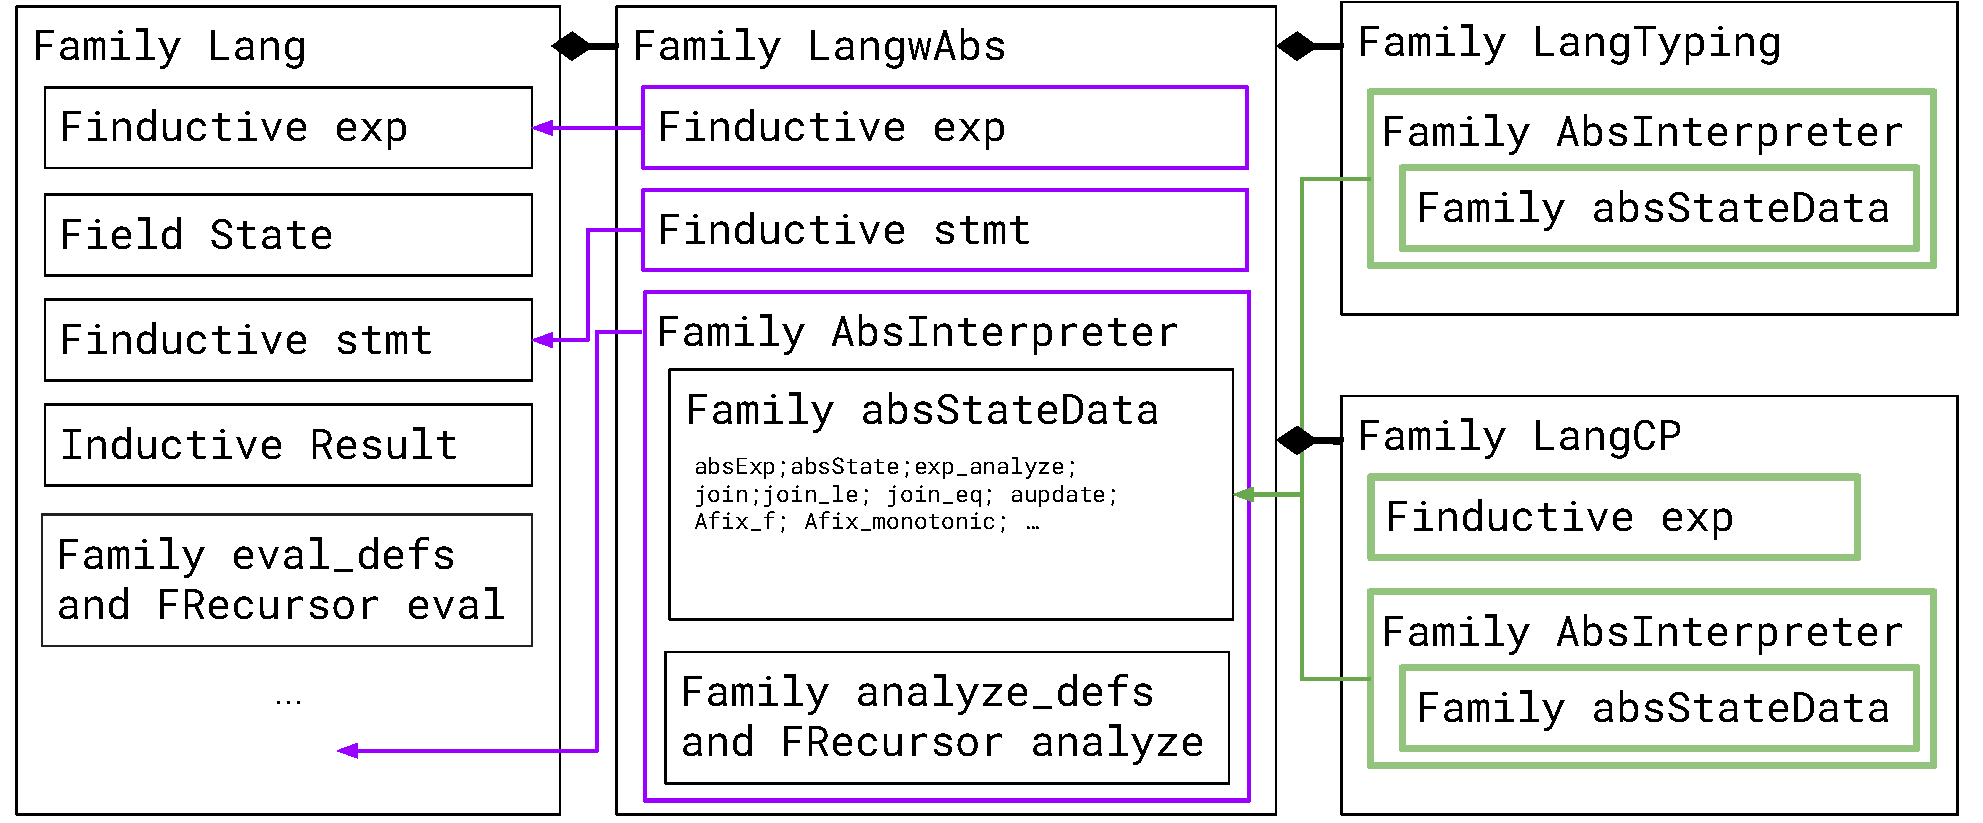
\includegraphics[width=\columnwidth]{coqexmaple/Family-Lang-Imp3.pdf}
  \caption{Inheritance Diagram for Abstract Interpretation Example. Black arrows are inheritance. Purple arrow are extending. Green arrows mean there are overriding.}\label{fig:abstract-interpretation-example}
\end{figure}

\begin{minted}[fontsize=\footnotesize]{Coq}
  Lemma analyze_faithful : forall prog st end_st, 
    interp prog st = end_st -> abs_interp prog (lift st) = (lift end_st)
\end{minted}
  

We construct four families, illustrated in \cref{fig:abstract-interpretation-example}.
The first family "Lang" define the big step operator (using fuel) of a
while language, with expression and stmt defined upon expression. Final "Result" can be error, "out-of-fuel" or a legitmate "State". It takes about 200 LOCs. 

The second family "LangwAbs" define the abstract interpreter for "Lang" in "LangwAbs.AbsInterpreter".
The idea of abstract interpretation is to lift concrete interpretation, their value and their states into their abstract correspondence. Then we come up with a faithful (one example would be "analyze_faithful") and generic abstract intepreter. Then, the user can freely choose the instantiation and lifting of this generic framework and end up with their aiming program analyzer. For example, lifting 1 into abstract value "integer" can give us a type inferer; lifting 1 into an element of a very flat lattice can gives us a constant propagator. There are also special mathematical structure required in the abstract value (like lattices) for the abstract interpretation. 

Thus, to implement this generic abstract interpreter, we need to postulate the abstract value and their mathematical property. Then we need to prove the abstract interpreter is \textbf{sound and terminating}  with the help of these postulations. Then for concrete analyzer, we only need to instantiate these postulation. The construction and proof of soundness uses "FInduction" and "FRecursion". "analyze_soundness" is saying if 
It takes about 300+ LOCs. 
% This example shows how
% to use family inheritance to extend a concrete interpreter with abstract
% interpreters. 
% This example also shows in this family polymoprhism framework we can reason about "Lang" with computation details being abstracted. 

% The third Family "LangMore" extend "LangwAbs" with nat constant and
% addition, and if-then-else control flow, of course retaining all the
% soundness theorem. It takes about 200+ LOCs. This is one example of
% using family inheritance to support new language feature, and compatible
% with the existent reasoning in "LangwAbs.AbsInterpreter". 

The third family and the fourth family "LangTyping" and "LangCP" instantiate the postulates of the
"LangwAbs" and recover computational information of "analyze". The corresponding fields in "absStateData" is overridden by concrete implementations. The resulting abstract interpreter is expected
to act as a type-analyzer and constant-propagator respectively. It takes about 200+ LOCs. 
% These are two examples of instantiate the detail computation of abstract interpretation. 


And at the end, the compiled module for "LangTyping" and "LangCP" is put into tests over simple queries. These "LangTyping" and "LangCP" also illustrates that we still have
computability in the presence of family.\YZ{Mention the alternative approach of using parameterized modules.}\EDJreply{What. I don't have that version. My earlier version without family is not extensible, just a POC to see if the proof idea itself is correct.}

\subsection{An Extensible Decision Procedure for Parsing}
\label{sec:coqexample-parser}
The third example is a decision procedure for parsing, based on the fact that, we can use Cop's Inductive Facility to encode CFG rules. Thus extensible inductive family corresponds to extensible CFG rules. For example, indexed type \mintinline{Coq}{is_prog : strs → Type} is a predicate asserting if a token list is a syntactically well-formed program.

\begin{figure}[!htb]
  \lstset{
      basicstyle=\fontsize{8}{8.5}\ttfamily,
  % numbers=left,
  }
  
  \begin{minipage}{\textwidth}
  \begin{multicols}{2}
  

  \definecolor{codecomment-color}{HTML}{0DA3FF}
  
  \begin{lstlisting}
  FInductive is_prog : strs -> Type := 
  | ip_seq : forall a b, is_prog a -> is_prog b 
      -> is_prog (a ++ [";"] ++ b) 
  | ip_assign : forall i e, is_atom i -> is_exp e 
      -> is_prog ([i; "="] ++ e).  
  \end{lstlisting}
  
  % \makeline[0pt]{Parser-exmp-before-start}{Parser-exmp-before-end}[codecomment-color!50]
  
  \columnbreak
  \definecolor{codecomment-color}{HTML}{5D030F}
  
  \begin{lstlisting}
  FInductive is_prog : strs -> Type += 
  | ip_if : forall a b, is_exp a -> is_prog b 
      -> is_prog (["if"] ++ a ++ ["then"] ++ b). 
  \end{lstlisting}
  
  
  
  % \makeline[.5\textwidth+9pt]{Parser-exmp-after-start}{Parser-exmp-after-end}[codecomment-color!50]
  
  \end{multicols}
  \end{minipage}
  \caption{"is_prog" and its extension}
  \end{figure}



We prove decidability of "is_prog" via strong induction on the length. The non-trivial part is  the inductive step, i.e. we need to show "is_prog" is ``conditionally decidable'':
\begin{minted}[fontsize=\footnotesize]{Coq}
  (forall e, len e < len s -> (is_prog e) + (is_prog e -> False)) -> (is_prog s) + (is_prog s -> False)
\end{minted}

This proposition should hold due to the shape of the inductive definition---because we can translate the definition of "is_prog" into an equivalence to a big disjunction: 
\begin{minted}[fontsize=\footnotesize]{Coq}
(∃ a ∃ b , is_prog a /\ is_prog b /\ s = a ++ [";"] ++ b)
\/ (∃ i ∃ e, is_atom i /\ is_exp e /\ s = i ++ [":="] ++ e) 
... 
<-> is_prog s
\end{minted}
Then decidability is immediate via this equivalence, since on LHS every sub token list has length strictly smaller than "s". 

However, when maintaining this equivalence proof through out different families---calling this big disjunction on LHS as \mintinline{Coq}{alg_is_prog : strs -> Type}---"alg_is_prog" is changing when "is_prog" extends. Thus "alg_is_prog" should be encoded as an overridable field. 

We will have challenges maintaining this equivalence proof. From left to right (soundness), we can have incremental construction and proof reuse throughout different families---we can easily prove "is_prog l" using each constructor. However, from right to left (completeness), the proof from the parent family cannot be reused in the children as "alg_is_prog" is changing and the proposition itself is changing. So we use "overridable" to organize the proof of completeness. 

It is around 750 lines of codes using Family facility and around 900 lines of code using vanilla Coq. Around 350 lines of them are public helper function used by both implementations.

% Then we provide an overridable predicate \mintinline{Coq}{alg_is_prog : strs -> Type},\YZ{Why does it need to be overridden?}\EDJreply{Basically alg_is_prog is a big disjunction list, corresponding to each of the constructor of }
% decidable provided the inductive hypothesis and sound \& complete w.r.t. to the specification \mintinline{Coq}{alg_is_prog e  <-> is_prog e}.  "alg_is_prog e" will be a big disjunction, of which each disjunct $P_i$ corresponds to the argument of one constructor of "is_prog" (each CFG rule). Thus once "is_prog" is extended, we need to disjunct "alg_is_prog" with more condition, thus overridable.  We require extension to take care of the disjuncts, their soundness \& completeness and the conditional decidablity.

% Among them, completeness \mintinline{Coq}{is_prog e -> alg_is_prog e} is
% the most challenging part. This is proved by recursion on the predicate
% "is_prog e", but none of the handler on "is_prog" will be reused
% because \mintinline{Coq}{alg_is_prog e} is overriden during
% inheritance.


% Unlike completeness, other parts of the construction, including
% soundness and and conditional decidability can be reused easily.
\YZ{But is the reusability achieved through a derived family's reusing handlers in the base family? Doesn't sound like it because the induction seems to be on strs.}\EDJreply{to prove something like alg_is_prog e -> is_prog e is not doing induction on string. It is just unfolding definition. \\ 
alg_is_prog is a big disjunction, alg_is_prog e = p1 e \/ p2 e\/ ..., and during overriding this disunction list is increasing. \\
So we organize the program by proving ``p1 e -> is_prog e'', ``p2 e -> is_prog e''. Everytime this disjunction list is increasing during overriding, the old proof ``p1 e -> is_prog e'' is reused in the new .}
